% 2007 年辽宁卷文科第 18 题：直三棱柱 ABC-A1B1C1，∠ACB=90°，AC=BC=a；
%   D、E 分别为 AB、BC 中点，M 为 AA1 上一点，二面角 M-DE-A 为 30°。
% 来源 PDF：gaokaomath-src/普通高考/2007/2007辽宁文.pdf
% SHA-256：dea57d961deb93eaab8a69627e54830eae297f588721e5b3bc9dc3ca3e3ae7c6
% 原页：2007辽宁文.pdf 第 1 页（A3 三栏）第 3 栏，书页码 391。
% 重绘依据：按原页斜投影与 C1—D、C1—E、M—D、M—E 的虚实线重绘，
%   MA 只画到 AA1 的中部，示意 M 在棱上而非端点。
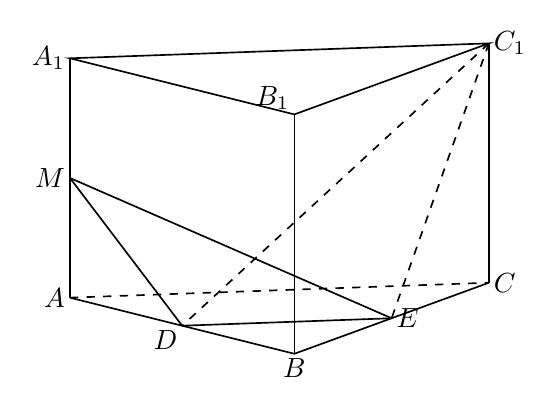
\begin{tikzpicture}[scale=0.95, semithick,
  every node/.style={inner sep=1.5pt}]

  \coordinate (A)  at (0,1.35);
  \coordinate (B)  at (3.0,0.60);
  \coordinate (C)  at (5.6,1.55);
  \coordinate (A1) at (0,4.55);
  \coordinate (B1) at (3.0,3.80);
  \coordinate (C1) at (5.6,4.75);
  \coordinate (D)  at (1.50,0.975);
  \coordinate (E)  at (4.30,1.075);
  \coordinate (M)  at (0,2.95);

  % 被遮挡的底边
  \draw[dashed] (A) -- (C);
  % 可见的底边与侧棱
  \draw (A) -- (B) -- (C);
  \draw (A) -- (A1);
  \draw (B) -- (B1);
  \draw (C) -- (C1);
  % 上底面
  \draw (A1) -- (B1) -- (C1) -- cycle;

  % 题设连线
  \draw[dashed] (C1) -- (D);
  \draw[dashed] (C1) -- (E);
  \draw (M) -- (D);
  \draw (M) -- (E);
  \draw (D) -- (E);

  \node[left] at (A) {$A$};
  \node[below] at (B) {$B$};
  \node[right] at (C) {$C$};
  \node[left] at (A1) {$A_1$};
  \node[above left] at (B1) {$B_1$};
  \node[right] at (C1) {$C_1$};
  \node[left] at (M) {$M$};
  \node[below left] at (D) {$D$};
  \node[right] at (E) {$E$};
\end{tikzpicture}
